\documentclass[12pt, a4paper]{article}
\usepackage[utf8x]{inputenc}
\usepackage{pdflscape}
\usepackage{graphicx}
\usepackage{geometry}
\usepackage{caption}
\usepackage{booktabs}
\usepackage{lipsum}
\usepackage{ragged2e}
\renewcommand{\contentsname}{İçindekiler Tablosu}
\renewcommand{\figurename}{Şekil}
\renewcommand{\refname}{Kaynakça}
\geometry{
	top=2.5cm,
	left=2.5cm,
	right=2.5cm,
	bottom=2.5cm
}
%opening
\title{AKILLI OTOPARK SİSTEMİ TASARIM DOKÜMANI}
\author{FARUK ÇETİN}

\begin{document}
	\begin{figure}[!ht]
		\centering
		
\includegraphics[
		width=40cm,
		height=10cm,
		keepaspectratio,
		]{logomuh.png}
		\maketitle
	\end{figure}
	\justify
	\frenchspacing
	\begin{abstract}
		This report presents in detail a smart car parking system design that aims to bring an innovative approach to traditional car parking systems. Aiming to provide a solution to the increasing vehicular traffic and car parking problems in modern cities, this project is realised by integrating special cameras including number plate reading technology and visual recognition features. The design aims to enable drivers to automatically recognise number plates, quickly identify empty car parking spaces and provide more efficient parking management. This innovative system aims to improve traffic flow and optimise urban transport while enhancing users' parking experience. By focusing on the details of the design process, the report reveals the key elements of this project, which has the potential to provide an advanced solution for smart car parking systems.
		
		\newpage
		\tableofcontents{} \newpage
		\section{GİRİŞ}
		Günümüzde şehirleşme ve artan araç sayısıyla beraber otopark yönetimi, her geçen gün daha karmaşık hale gelmektedir. Bu bağlamda, modern teknolojinin sunduğu fırsatları kullanarak geleneksel otopark sistemlerine getirilecek yenilikçi çözümlerle ilgili bir tasarım geliştirilmektedir. Proje kapsamında, plaka okuma teknolojisiyle donatılmış özel kameralar ve otoparktaki boş ve dolu yerleri anlık olarak gösteren bir kamera sistemi entegre edilerek otoparkları daha az insanla kontrol etmek  amaçlan\-maktadır. Bu akıllı otopark sistemi, sürücülere plakaları otomatik olarak tanıma ve otoparktaki boş alanları kolayca bulma imkanı sunarak otopark deneyimini daha verimli ve kullanıcı dostu bir hale getirmektedir. Böylece, sürücülerin otopark alanlarını etkin bir şekilde kullanmalarını sağlamak, trafik akışını iyileştirmek ve şehir içi ulaşımı daha sürdürülebilir hale getirmek için tasarlanmış bu proje, modern şehir yaşamına katkı sağlamayı hedeflemektedir.
		\section{Literatür Araştırması}
		Akıllı otopark sistemleri şehirlerin trafiğini yönetmek ve otopark yerlerinin etkin bir şekilde kullanılmasını sağlamak amacıyla önemli bir teknolojik gelişme alanıdır. Araştırmacılar, gelişen görüntü işleme teknolojileri ve yapay zeka yöntemleri ile plaka tanıma sistemlerini geliştirerek, otopark girişlerindeki trafiği yönetmek için etkili çözümler sunmaktadırlar. Özellikle derin öğrenme tekniklerinin kullanımıyla, plakaların yüksek doğrulukla tanınması ve veritabanlarına hızlı bir şekilde aktarılması sağlanmaktadır. Ayrıca, kamera sistemlerinin kullanımıyla otopark alanlarının boş ve dolu yerlerinin gerçek zamanlı olarak izlenmesi ve bu bilgilerin merkezi bir veritabanına aktarılması, akıllı otopark yönetimi için önemli bir adımdır. Bu veritabanı, sürücülere boş park yerlerini hızlıca bulmaları için yönlendirme yaparken, otopark işletmecilerine de doluluk oranları ve trafiği analiz etme imkanı sunmaktadır. Bu bağlamda, literatürdeki araştırmalar, akıllı otopark sistemlerinin geliştirilmesi ve optimize edilmesi için değerli bilgiler sağlamaktadır.
		\cite{ozdemir2020guvenlik} 
		\cite{dougarougluakilli}
		Bu projelerde kullanılan teknolojiler örnek alınarak proje planı oluşturulmaya çalışılmıştır. Servo motor ve mikrodenetleyici kullarak sistemin nasıl tasarlanması gerektiği açıklanmıştır.
		 
		\subsection{Benzer Yapılmış Çalışmalar}
		Geleneksel otopark yönetim sistemlerine kıyasla daha verimli ve kullanıcı dostu bir yaklaşım sunan akıllı otopark sistemleri; genellikle bir dizi sensör, yazılım ve veri analitiği aracılığıyla otopark yönetimini optimize ederler. Sensörler, genellikle yeraltı dedektörleri, kameralar veya lazerler gibi çeşitli teknolojileri içerir ve araçların park yerlerini tespit etmek için kullanılır\cite{article_1098978}. Otomatik Otopark Sistemi (OOS), sürücülerin araçlarını girişte bıraktıkları ve
mekanik olarak otopark tarafından düşey ve yatay hareketler ile aracın uygun park
yerine taşındığı bir bilgisayar kontrollü sistemdir. Sistem
sınırlı sayıdaki otopark alanının azami düzeyde kullanılmasını sağlar. Bu sistemde,
sürücülerin otoparkın içerisine girmeleri gerekmediği için park etme süresi ve
güvenlik konusunda daha etkin hizmet sunulmaktadır\cite{dougarougluakilli}.
Açık dinamik otoparklar ve kapalı dinamik otoparklarda da uygun park alanlarının tespit edilmesi için kullanılan dijital sistemler farklılık göstermektedir. Açık dinamik otoparklarda, uygun park alanlarının saptanması için otopark genelini görüntüleyebilecek kameralardan yararlanılırken kapalı dinamik otoparklarda ise her park alanının üzerine araç algılayıcı sensörler yerleştirilerek araçlar tespit edilmektedir\cite{article_1252682}.

		\section{Metodoloji}
		Bu bölümde projenin nasıl yapılacağı ve projede neler kullanılacağı anlatılmaktadır.
		\subsection{Akıllı Otopark Projesi Nedir?}
		Günümüzde şehirlerdeki artan araç sayısı ve bu artışın getirdiği otopark yönetim zorluklarını oluşturmuştur.Bu bağlamda, "Akıllı Otopark Sistemi" projesi ,sürücülere daha etkin, hızlı ve güvenli bir otopark deneyimi sunmayı hedeflemektedir.
		
		Projenin temel amacı, plaka tanıma teknolojisi ile otoparkın dolu ve boş yerlerini anlık olarak göstererek boş olan park bölgelerine araçları yönlendirip zaman kaybını minimize etmeyi hedefler. 
		
		Proje, şehir içi trafiği azaltmayı, park alanlarının daha etkili bir şekilde kullanılmasını sağlamayı ve güvenlik standartlarını artırmayı amaçlamaktadır.
		
		\subsection{Plaka Tanıma}
			\begin{figure}[!htbp] %[h]
			
			\centering
			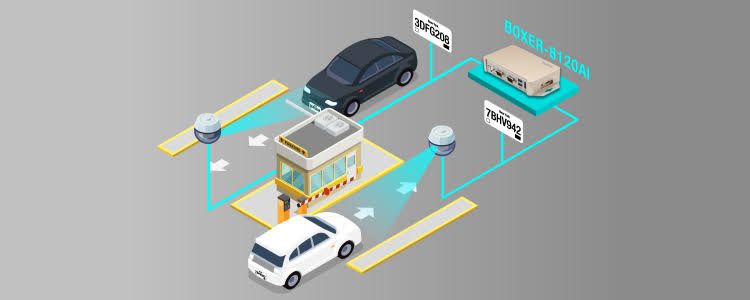
\includegraphics[
			width=13cm,
			height=13cm,
			keepaspectratio,
			]{bariyer.jpg}
			\caption{Örnek Otopark Girişi}
		\end{figure}
		Projede plaka tanımlamak için takip edilecek adımlar:
		
		\subsubsection{Gerekli Kütüphanelerin Kurulumu}  Proje Python programla dili üzerinde yapılacaktır. Pythonun kütüphaneleri olan: OpenCV, NumPy ve Matplotlib kurulumunu gerçekleştirilecektir. Bu kütüphaneler, görüntü işleme, veri manipülasyonu ve grafiksel görselleştirme işlemleri için gereklidir.
		\subsubsection{Veri Toplamau}Plaka tanıma algoritmasını eğitmek ve test etmek için bir veri setine ihtiyacımız olacaktır. Bu aşamada, farklı araç plakalarının görüntülerini içeren bir veri seti toplanmaktadır. Ayrıca, plakaların konumunu etiketlemek için gerekli olan bilgileri elde etmek için manuel olarak plakalar belirlenmektedir.
		\subsubsection{Plaka Tanıma Modelinin Eğitimi}Veri setini kullanarak plaka tanıma modeli eğitilecektir. Cerry algoritmasını kullanarak plakaların görüntüleri oluşturulacaktır ve bu görüntülerin üzerinde özellik çıkarma ve sınıflandırma işlemlerini gerçekleştirilecektir. Eğitim süreci boyunca, modelin doğruluğunu artırmak için hiperparametre ayarlaması yapılabilecektir.
		\subsubsection{Modelin Değerlendirilmesi}Eğitim sürecinin ardından, model performansı değerlendirilecektir. Bu adımda, ayrı bir test veri seti kullanılarak modelin doğruluğunu, hassasiyetini ve geri çağırma oranı hesaplanacaktır. Ayrıca, yanlış sınıflandırılan plakalar görsel olarak incelenerek modelin zayıf noktaları belirlenecektir.
		\subsubsection{Akıllı Otopark Sistemi Entegrasyonu}Başarıyla eğitilmiş plaka tanıma modeli, akıllı otopark sisteminin bir parçası olarak entegre edilecektir. OpenCV kütüphanesi kullanılarak kamera görüntülerini yakalanacak ve bu görüntüler üzerinde plaka tanıma işlemleri gerçekleştirilecektir. Tanınan plakaların veritabanına gönderilmesi de bu işlemlerden sonra yapılacaktır.
		\subsubsection{Boş/Dolu Park Yerlerinin Belirlenmesi} Opencv kütüphanesi kullanarak kamera görüntülerini analiz ederek, otopark alanındaki boş ve dolu park yerlerini tespit edilecektir. Bu bilgiler bir veritabanına kaydedilerek sürücülere yönlendirilme yapılmak üzere kullanılacaktır.
		\subsubsection{Sonuçların Değerlendirilmesi} Akıllı otopark sistemi üzerinde gerçekleştirilen işlemlerin sonuçlarını değerlendirilecektir. Sistemin etkinliğini ve performansını ölçmek için belirlenen kriterleri kullanılarak sistemin otopark trafiğini yönetme ve kullanıcı deneyimini iyileştirme yeteneğini hesaplanacaktır.
		
		\subsection{Boş/Dolu Park Yeri Belirleme}
			
			\begin{figure}[!htbp] %[h]
			\centering
			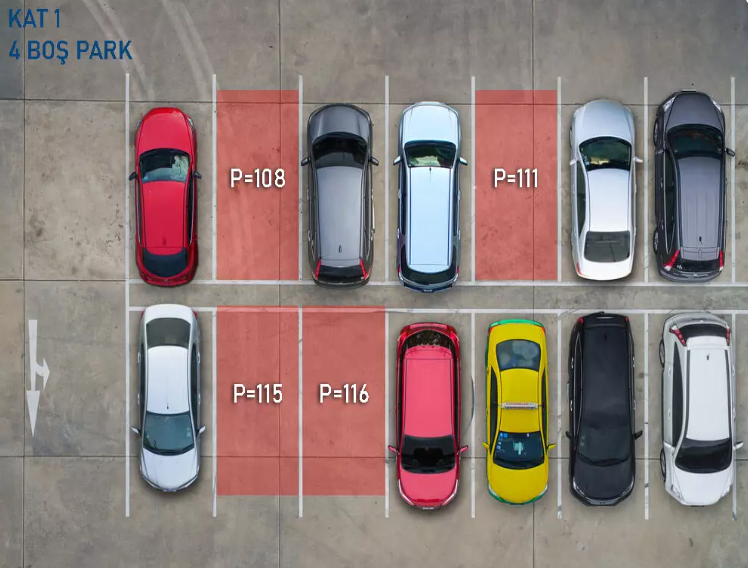
\includegraphics[
			width=11cm,
			height=11cm,
			keepaspectratio,
			]{park.png}
			\caption{Örnek Boş/Dolu Takibi}
		\end{figure}
		Bu aşamada, akıllı otopark sisteminin temel bileşenlerinden biri olan boş/dolu park yerlerinin belirlenmesi süreci ele alınacaktır.
		\subsubsection{Görüntü İşleme ve Nesne Tanıma} Opencv kütüphanesi kullanılarak, kamera tarafından sağlanan canlı görüntüler üzerinde nesne tanıma ve görüntü işleme algoritmaları uygulanacaktır. Bu adımda, görüntüden otomatik olarak park yeri tespit edip dolu ve boş yerler belirlenecektir. Daha sonra bu bilgiler bir veri tabanına kaydedilecektir.
		\subsubsection{Hesaplama ve Analiz} Her karedeki değişikliklerin takibi yapılacak ve bir önceki kare ile karşılaştırılarak boş ve dolu park yerlerinin belirlenmesi sağlanacaktır. Hareket algılama algoritmaları kullanılarak araçların giriş ve çıkışları tespit edilerek bu bilgiler veri tabanına kaydedilecektir.
		\subsubsection{Grafiksel Gösterim ve Arayüz} Matplotlib kütüphanesi kullanılarak, otopark haritası oluşturulacak ve bu harita üzerinde boş ve dolu yerler görselleştirilecektir.
		\subsubsection{Gerçek Zamanlı İzleme ve Güncelleme} Görüntü işleme algoritmaları gerçek zamanlı olarak çalışacak ve herhangi bir değişiklik algılandığında veri tabanı güncellenecektir. Bu sayede, kullanıcılar otoparktaki mevcut durumu anlık olarak takip edebileceklerdir.
		\subsubsection{Performans Değerlendirmesi} Geliştirilen algoritmaların performansı, doğruluk ve hız açısından değerlendirilecektir. Bu değerlendirme sürecinde, sistem tarafından belirlenen boş/dolu park yerleri ile gerçek durum karşılaştırılacak ve sistem doğruluğu ölçülecektir. Ayrıca, algoritmaların işleme süreleri ve sistem cevap hızı da değerlendirilerek gerekirse iyileştirmeler yapılacaktır.
		
		
		\begin{landscape}

			\begin{figure}[!htbp] %[h]
			
				\centering
				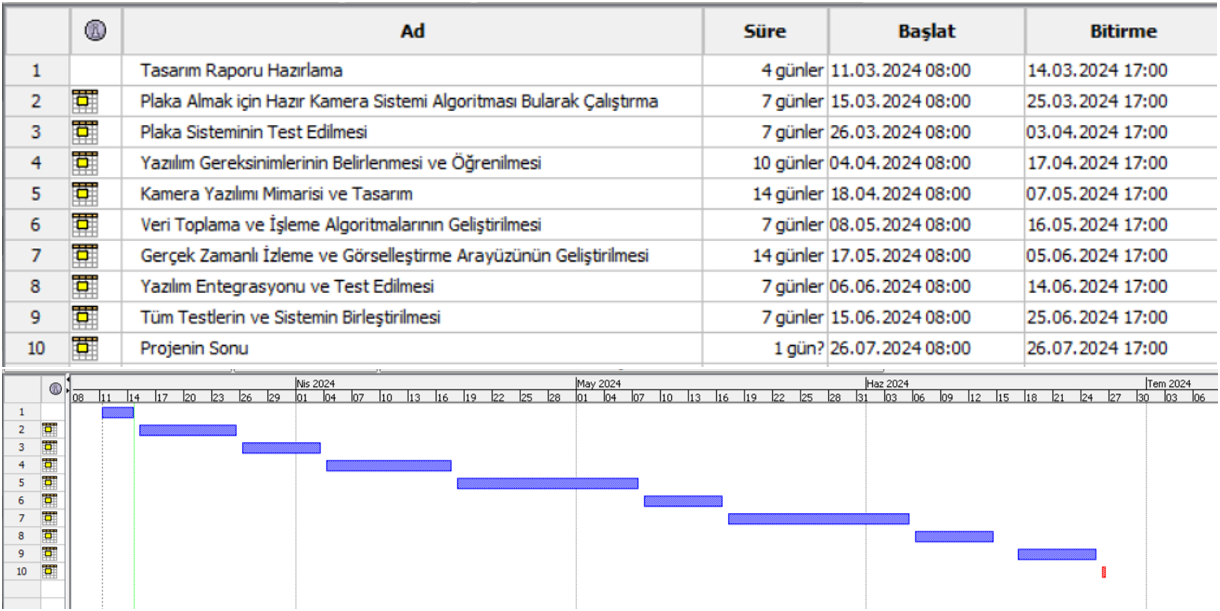
\includegraphics[
				width=30cm,
				height=30cm,
				keepaspectratio,
				]{gantchart.png}
				\caption{Gantt Chart}
			\end{figure}		
		\end{landscape}
					\newpage
		Bu Gantt Chart şeması, akıllı otopark sistemi projesinin ana aşamalarını detaylı bir şekilde göstermektedir. İlk aşama olan "Literatür Araştırması Yapma", mevcut teknolojik gelişmeleri ve benzer projeleri değerlendirme sürecini içerir. "Tasarım Raporu Hazırlama" aşamasında, proje tasarımının detayları belirlenir ve planlama raporu oluşturulur. "Plaka Kamera Sistemi Algoritması" aşamasında, plaka okuma için hazır bir veri seti ile yapılmış çalışma bulunur ve çalıştırılır.
		
		"Plaka Sistemi Testi" aşamasında, seçilen sistem test edilir. Ardından, "Doluluk Oranı Kamera Algoritması" aşamasında otoparkta doluluk oranını belirlemek için bir algoritma yazılır. Bu algoritma, "Algoritmanın Testi ve Geliştirilmesi" aşamasın\-da detaylı bir şekilde test edilir ve geliştirilir.
		
		"Tüm Testler ve Sistemin Birleştirilmesi" aşamasında, tasarlanan tüm bileşenler birleştirilir ve bütün sistem geniş kapsamlı bir şekilde test edilir. Proje, "Projenin Sonu" aşamasında tamamlanır ve kullanıma hazır hale getirilmek üzere diğer aşama\-lara geçilerek sistem geliştirilmesi için yeni bir proje olarak geliştirilmesi sağlanır.
		
	\begin{figure}[!htbp] %[h]
	\centering 
	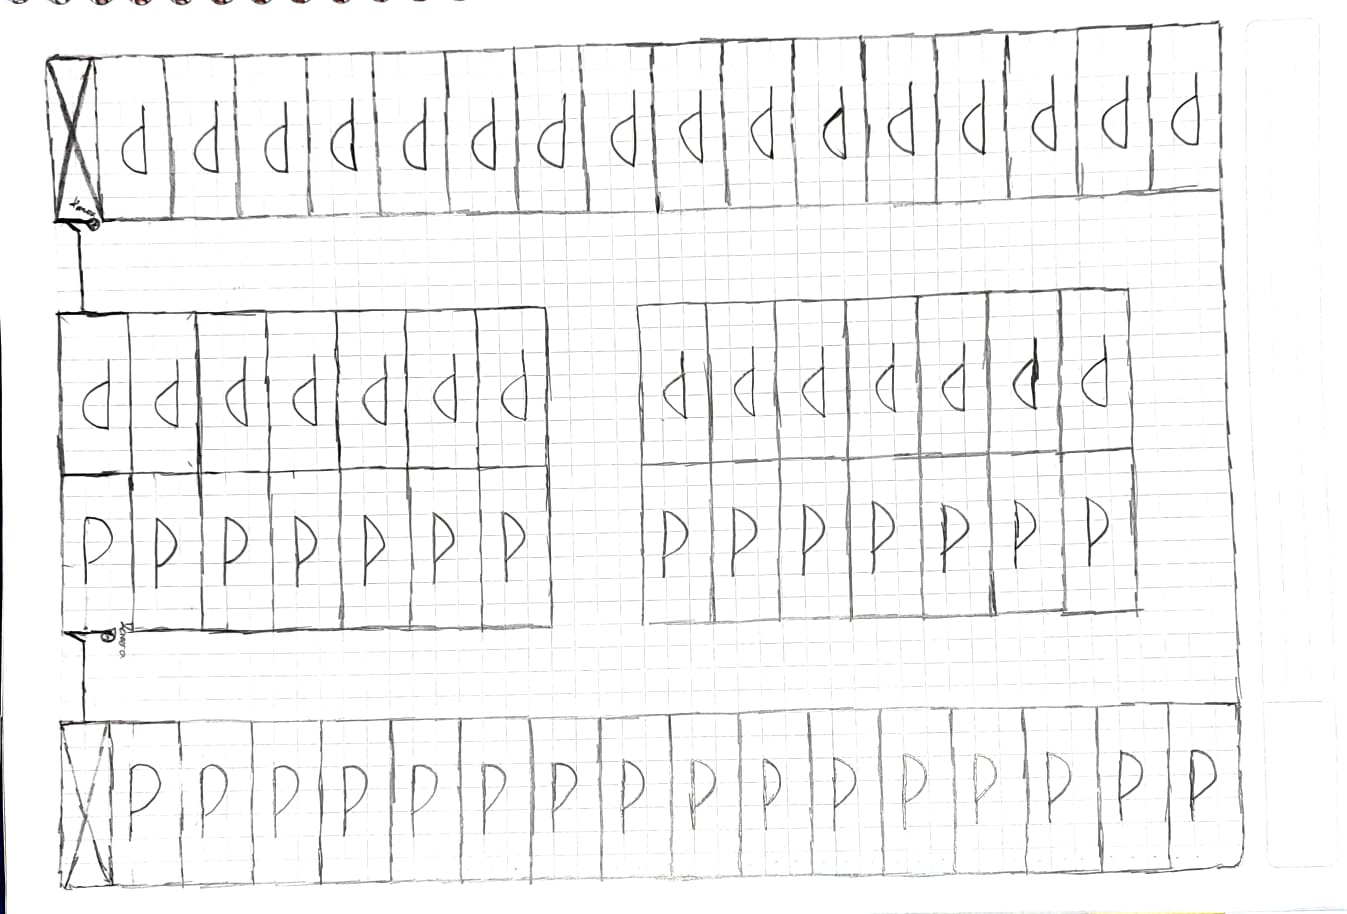
\includegraphics[
	width=9cm,
	height=9cm,
	keepaspectratio,
	]{Otopark_Taslak} 
	\caption{Otopark Taslağı}
	\label{OtoparkTaslagi}
\end{figure}
Bu [\ref{OtoparkTaslagi}] otopark taslağı projemizde kullanılacak olan yerin örnek çizimidir.

\begin{figure}[!htbp]
	\centering 
	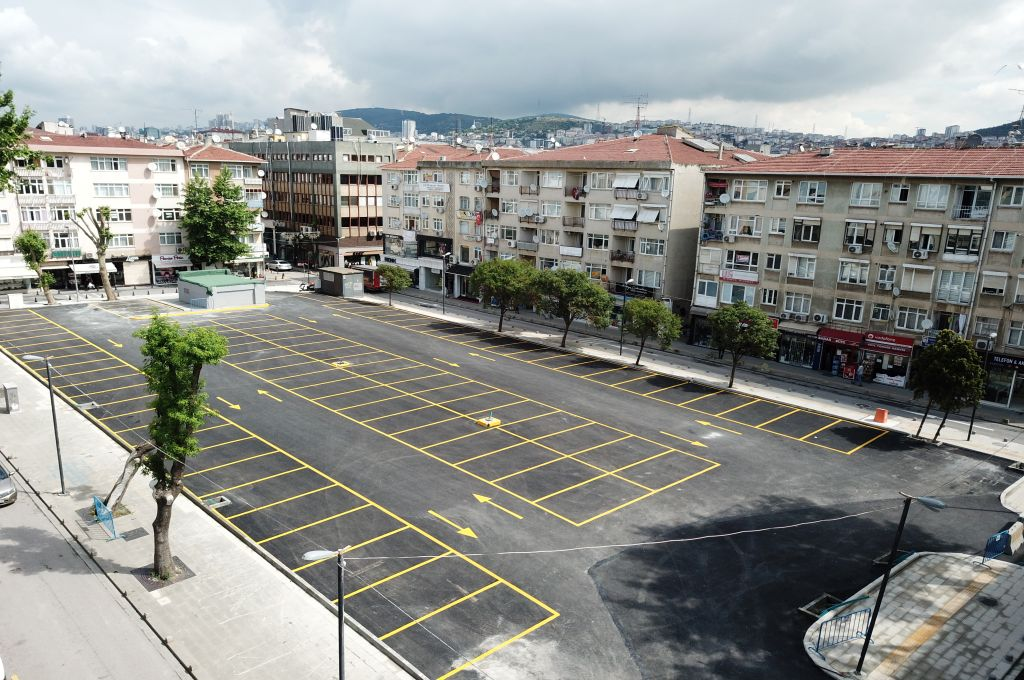
\includegraphics[
	width=9cm,
	height=9cm,
	keepaspectratio,
	]{OrnekPark} 
	\caption{Örnek Bir Otopark}
	\label{OtoOrnek}
\end{figure}

Bu [\ref{OtoOrnek}] otopark resmi projemizde kullanılacak olan otaparkın gerçek bir örneğidir ve farklı bir kaynaktan alınmıştır.

		\section{VeriTabanı ve Veriler}
		Projemizde ilk önce hazır ve az olan bir dataset kullanılacaktır.
			\begin{figure}[!htbp] %[h]
			\centering 
			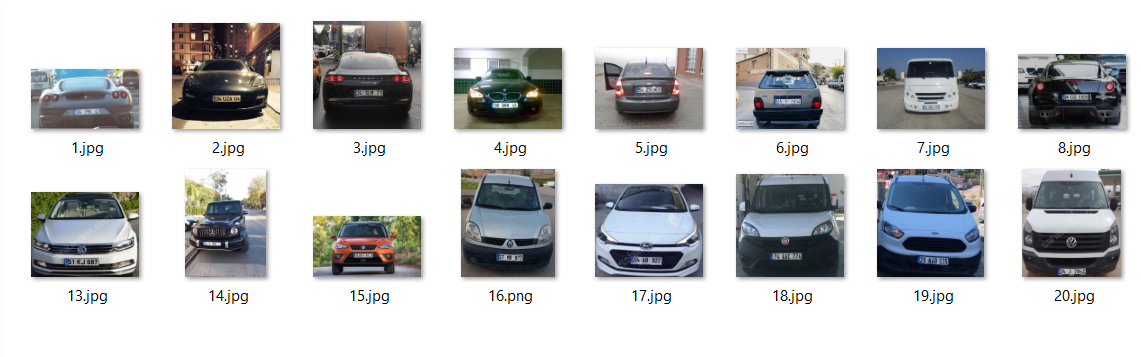
\includegraphics[
			width=13cm,
			height=13cm,
			keepaspectratio,
			]{Veri.png}
			\caption{Hazır Dataset}
		\end{figure}
		
		Veriler istenilen etkiyi sağlamaz ya da sorunlar çıkartırsa kaggleda bulunan datasetlere bakılarak yeni bir dataset oluşturulacaktır.
		\section{Beklenen Sonuçlar}
		
		\begin{figure}[!htbp] %[h]
			\centering 
			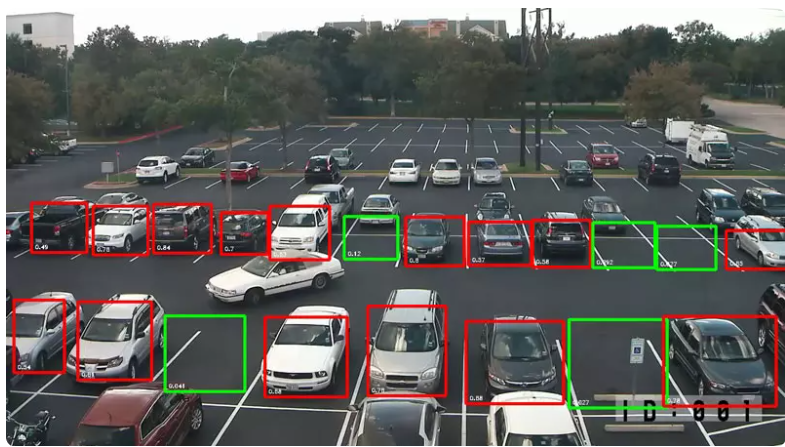
\includegraphics[
			width=13cm,
			height=13cm,
			keepaspectratio,
			]{AkilliOto.png}
		\end{figure}
		Bu akıllı otopark sistemi projesinin başarıyla tamamlanması beklenen bir dizi olumlu sonucu beraberinde getirecektir. Öncelikle, plaka okuyan kamera sistemimizin yüksek hassasiyetle çalışması ve hızlı bir şekilde giriş-çıkış işlemlerini gerçekleştirmesi, sürücü\-lere otopark içindeki hareketlilikleri daha etkin bir şekilde yönetme imkanı sunacaktır. Bu, özellikle yoğun trafik saatlerinde ve otoparklarda hızlı geçişlerin daha hızlı bir şekilde yapılmasını sağlayarak sürücülerin zaman tasarrufu yapmalarına olanak tanıyacaktır.
		
		Ayrıca, otopark alanındaki kameraların boş ve dolu park yerlerini doğru bir şekilde tespit etmesi, kullanıcılara gerçek zamanlı olarak park yerlerinin durumunu göstererek boş alanları kolayca bulmalarına yardımcı olacaktır. Ayriyeten otoparkın dolu olması durumunda da girişe izin vermeyeyek sürücülerin otopark içindeki dolaşım süreçlerini optimize etmelerini sağlayarak trafik sıkışıklığını ve karışıklığı azaltacak ve genel otopark deneyimini iyileştirecektir.
		
		Giriş-çıkışların kontrolü ve servo motor aracılığıyla kapı açma/kapama sisteminin entegrasyonu sayesinde, plaka tanıma sistemi tarafından tanımlanan araçların güvenli bir şekilde giriş ve çıkışları sağlanacaktır. Bu durum, otopark güvenliğini önemli ölçüde artırarak yetkisiz girişleri engelleyecektir.
		
		Akıllı otopark sistemi, kullanıcı dostu bir arayüzle entegre edilecektir. Sürücüler, mobil veya web uygulaması üzerinden otoparktaki boş alanları görebilecek, giriş-çıkış işlemlerini kolayca yönetebilecek ve sistemden anlık bilgiler alabileceklerdir. Bu, sürücülerin otopark deneyimini daha interaktif ve kontrol edilebilir kılacak, kullanım kolaylığını artıracak ve müşteri memnuniyetini yükseltecektir.
		
		Sonuç olarak, bu projenin başarıyla uygulanması, otopark yönetimini daha etkin, sürücülerin otopark içindeki hareketliliğini daha akıcı hale getiren bir çözüm sunacak ve şehir içindeki trafik akışını optimize edecektir. Bu, sürdürülebilir ve konforlu bir şehir yaşamına katkı sağlayarak aynı zamanda güvenlik standartlarını da artıracaktır.
		
		\bibliographystyle{ieeetr}
		\bibliography{references.bib}
		\dots{}
		
		
	\end{abstract}
	
\end{document}
